\documentclass[11pt,a4paper]{article}
\usepackage[hyperref]{acl2018}
\usepackage{amsmath}
\usepackage{graphicx}
\usepackage{amsfonts}
\usepackage{times}
\usepackage{latexsym}

\usepackage{url}

\aclfinalcopy

\title{Using Geospatial Data to Find Investment Opportunities in the Real Estate Market}

\author{Chih Huang \\
  {\tt huangcs} \\
  {\tt @seas.upenn.edu} \\\And
  Ignacio Navarro \\
  {\tt inavarro} \\
  {\tt @seas.upenn.edu} \\\And
  Nikhil Ramesh \\
  {\tt nramesh} \\
  {\tt @seas.upenn.edu}
}

\date{\today}

\begin{document}
\maketitle
\begin{abstract}
  Valuating real estate properties is driven by a series of direct 
  factors (total square area, number of bedrooms, garage spaces, etc) 
  and indirect factors (crime rate, quality of school district, etc). However, private sellers tend to focus more on the former when setting 
  a listing price for their property. In particular, there are many
  geospatial features indirectly related to the property that sellers
  might easily overlook. Proximity to a church, a river, or a police
  station are all factors that play a role, albeit minor, in the valuation
  of a property. In this paper we determine by running a series of models on a dataset consiting
  on properties in South Philadelphia if geographical features do indeed play a decisive role 
  in the valuation of a property. 
\end{abstract}

\section{Introduction}

\subsection{Motivation}

Traditionally, real estate valuation has concentrated on assessing the
features directly surrounding the property to come up with a price.
Straightforward features such as number of bedrooms, whether the property
has a pool or a garage space, or even the number of bathrooms play a major
contribution on the price. And while that makes perfect sense, private
sellers may not fully realize that the property's surroundings can also
play a role. Points of interest like supermarkets, museums, parks, cafes,
or police stations can affect house prices but many times these may be
overlooked. 

\subsection{Problem Definition}

With all of this in mind the natural question becomes: given all the 
geospatial data related to a property, can a machine learning model 
predict the real value of a property as a \textbf{regression} problem? 
And if so, can one use this to
find investment opportunities in the real estate market? Throughout
this paper we will answer the former question. The latter is a simple
corollary of the former. Indeed, if there is a model that can accurately 
predict house prices given geospatial and direct features, one can use these
results to find investments opportunities by comparing the listing
price on properties currently on the market with what the best model 
predicts the value is and seeing if the property is really undervalued.

\medskip

In other words, let $M: X \to \mathbb{R}^+$ be an accurate model (we will
define what constitutes ``accurate'' to our use case in the next section),
where $X$ is the feature space that constitutes direct and indirect
features related to a property. Given a property $p$ with a listing price of $s_p$ and a set of features $x_p$, we will buy the property if

\begin{equation}
  M(x_p) > s_p
\end{equation}

because $p$ is undervalued.

\subsection{Related Work}

A lot of work has been done in the last few years on predicting house prices
using machine learning. Traditional models have relied in hedonic
regression, a type of regression which breaks the property apart into its direct factors in order to establish
a relationship between the factors and the price of the property. A paper using this method have been 
presented by \cite{jiang2014new} focusing on properties in Singapore with property sales between 1995 and 2014.

\medskip

Our main source for our project is \cite{bergadano2019learning},
in which they analyze a dataset consiting of properties in Madrid, Spain.
There are similarities to what we're trying to investigate: the paper models
the question as a regression problem and uses similar models to the ones we train. 
The main difference, however, is that they only consider direct features for their models. 
The main novelty in our project is to combine these features with geospatial features.
As far as we have researched, no work has investigated our proposal.


\section{Data Acquisition and Exploration}

\subsection{Acquisition}

The acquisition of the dataset for this project consisted on finding basic property
information for Philadelphia that included direct features, and merging this dataset
with all the geospatial information related to the property. The first part was
relatively easy, as \url{https://www.opendataphilly.org/} provided basic information
for over 250,000 properties in Philadelphia. The main challenge was in fact finding
the geographical features. Our approach to solve this was to find APIs that offered
nearest distance to points of interests. Once we found some reliable APIs for this task
(e.g. GoogleMaps API, TomTom API, or FourSquare API), we began the process of merging
the data to our property dataset.

\medskip

The main obstacle of this part, and probably of the project,
was the API rate limit each service offered. Conservatively
speaking, we needed to make
$$
\underbrace{250,000}_{\text{properties}} \times
\underbrace{24}_{\text{geo features}} = 6,000,000 \; \text{API calls}
$$
and unfortunately most of the services offered 1,000 API
calls limit per day. The solution to this part was to
drastically reduce the size of the dataset to around
8,000 properties in South Philadelphia, and even this
amount posed some architectural challenges: we distributed
the API calls for each member of the group and remerged them later. We encourage the reader to look at the code dealing
with this on the project's \href{https://github.com/nachonavarro/real-estate-ml}{repo}, in particular 
the \texttt{properties/data} package.

\subsection{Features}

The list of final features that we feed our model are in
Table \ref{tab:features} for a total of 5 categorical
and 28 numerical.

\begin{table}[]
\centering
\begin{tabular}{|l|l|}
\hline
\textbf{Feature} & \textbf{Type} \\ \hline
Fireplaces       & categorical   \\ 
Garage Spaces             & categorical \\ 
Bathrooms                 & categorical \\ 
Bedrooms                  & categorical \\ 
Stories                   & categorical \\ 
Total Area                & numerical   \\ 
Total Livable Area        & numerical   \\ 
Latitude                  & numerical   \\ 
Longitude                 & numerical   \\ 
Nearest Museum            & numerical   \\ 
Nearest Gas Station       & numerical   \\ 
Nearest Coffee Shop       & numerical   \\ 
Nearest Stadium           & numerical   \\ 
Nearest Food              & numerical   \\ 
Nearest Bar               & numerical   \\ 
Nearest Gym               & numerical   \\ 
Nearest Bridge            & numerical   \\ 
Nearest Garden            & numerical   \\ 
Nearest Park              & numerical   \\ 
Nearest River             & numerical   \\ 
Nearest City Hall         & numerical   \\ 
Nearest Police Station    & numerical   \\ 
Nearest Hospital          & numerical   \\ 
Nearest Elementary School & numerical   \\ 
Nearest Church            & numerical   \\ 
Nearest Bank              & numerical   \\ 
Nearest Supermarket       & numerical   \\ 
Nearest Pharmacy          & numerical   \\ 
Nearest Bus Stop          & numerical   \\ 
Nearest Metro Station     & numerical   \\ 
Nearest Train Station     & numerical   \\ 
Nearest University        & numerical   \\ 
Nearest Laundromat        & numerical   \\ \hline
\end{tabular}
\caption{Features used}
\label{tab:features}
\end{table}

\subsection{Exploration}

Once we acquired the data the next step was to explore it
to fully understand it. Some significant results to show are
the following.

\medskip

The distribution of the properties by sale price in South Philadelphia can be seen in Figure \ref{fig:distribution}.
Clearly the distribution is skewed with a mean sale
price of \$324,662.

\begin{figure}[h]
\centering
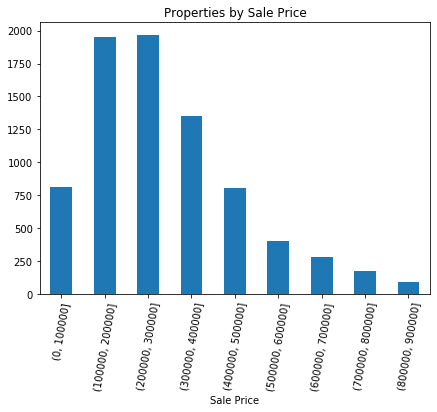
\includegraphics[width=0.5\textwidth]{properties_sale_price}
\caption{Distribution by sale price}
\label{fig:distribution}
\end{figure}

We can also get a sense of where the properties are located
by plotting a heatmap of South Philadelphia based on
sale price (Figure \ref{fig:heatmap}).

\begin{figure}[h]
\centering
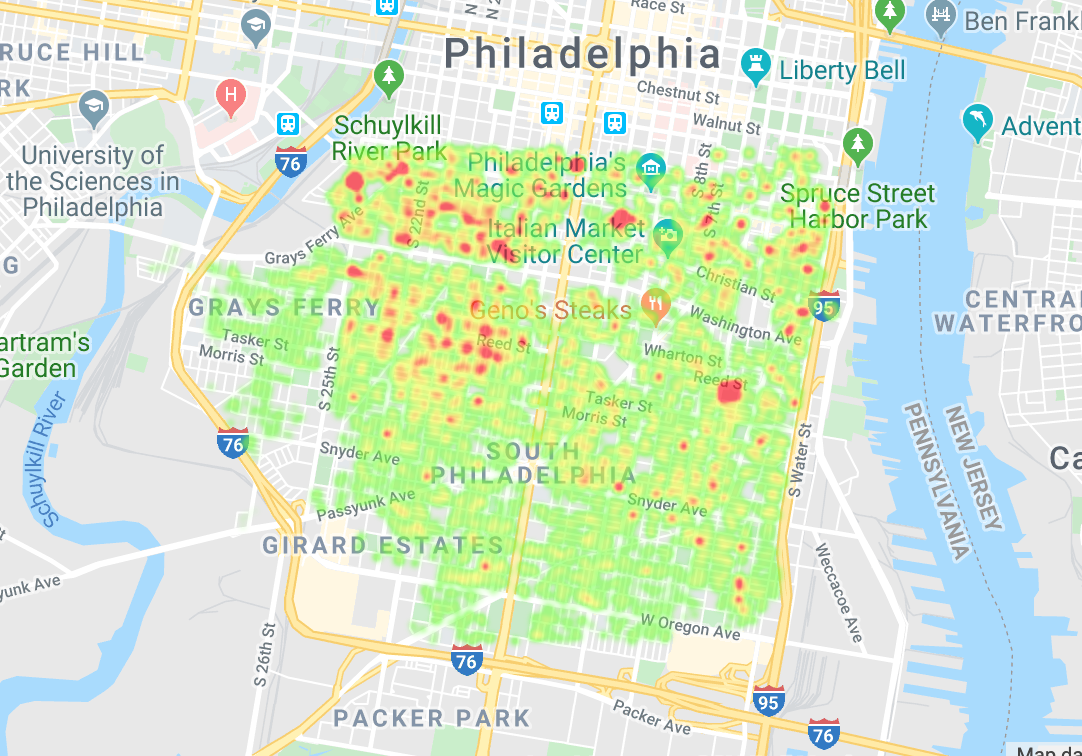
\includegraphics[width=0.5\textwidth]{heatmap}
\caption{Heatmap of South Philadelphia (hotter means higher
sale price)}
\label{fig:heatmap}
\end{figure}

Another important step was to see the relationship
between the features. To do this we used a correlation
matrix which can be seen in Figure \ref{fig:corr}. For instance, there is a strong correlation between the number of bathrooms and the total livable area. There's also some interesting relationships, e.g., there is negative correlation between the total livable area and the nearest laundromat, which makes (some) sense, as bigger houses in richer neighborhoods don't need laundromats.


\begin{figure}[h]
\centering
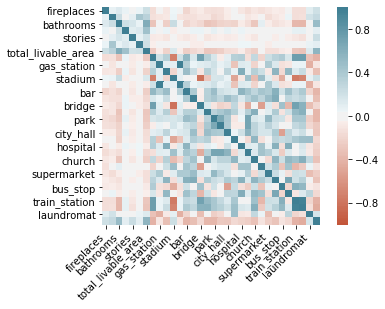
\includegraphics[width=0.5\textwidth]{correlation_matrix}
\caption{Correlation matrix}
\label{fig:corr}
\end{figure}


\section{Models}

Lorem ipsum dolor sit amet, consectetur adipisicing elit, sed do eiusmod
tempor incididunt ut labore et dolore magna aliqua. Ut enim ad minim veniam,
quis nostrud exercitation ullamco laboris nisi ut aliquip ex ea commodo
consequat. Duis aute irure dolor in reprehenderit in voluptate velit esse
cillum dolore eu fugiat nulla pariatur. Excepteur sint occaecat cupidatat non
proident, sunt in culpa qui officia deserunt mollit anim id est laborum.

Lorem ipsum dolor sit amet, consectetur adipisicing elit, sed do eiusmod
tempor incididunt ut labore et dolore magna aliqua. Ut enim ad minim veniam,
quis nostrud exercitation ullamco laboris nisi ut aliquip ex ea commodo
consequat. Duis aute irure dolor in reprehenderit in voluptate velit esse
cillum dolore eu fugiat nulla pariatur. Excepteur sint occaecat cupidatat non
proident, sunt in culpa qui officia deserunt mollit anim id est laborum.

\section{Conclusion}

Lorem ipsum dolor sit amet, consectetur adipisicing elit, sed do eiusmod
tempor incididunt ut labore et dolore magna aliqua. Ut enim ad minim veniam,
quis nostrud exercitation ullamco laboris nisi ut aliquip ex ea commodo
consequat. Duis aute irure dolor in reprehenderit in voluptate velit esse
cillum dolore eu fugiat nulla pariatur. Excepteur sint occaecat cupidatat non
proident, sunt in culpa qui officia deserunt mollit anim id est laborum.

\subsection{Future Work}


\bibliographystyle{acl_natbib}
\bibliography{acl2018}

\end{document}
